\chapter{Blok p I: Golongan Boron, Karbon, dan Nitrogen}\label{ch:b1:p-block-13-15}

Udara yang kita hirup terdiri atas empat perlima nitrogen, tetapi
tumbuhan kekurangan nitrogen: ikatan rangkap tiga \ce{N#N} begitu kuat
sehingga hampir tidak ada yang dapat memutusnya. Sepanjang sebagian besar
sejarah, nitrogen tanaman berasal dari pupuk kandang, dari bakteri yang
hidup pada akar kacang-kacangan, dan dari nitrat yang ditambang. Pada
awal abad kedua puluh, sebuah reaksi antara nitrogen dan hidrogen di atas
\omterm{def:b1:elementary-steps:catalyst}{katalis} besi mengubah keadaan itu; kini dunia membuat sekitar 160 juta
ton nitrogen setahun dalam bentuk amonia, dan kira-kira separuh nitrogen
dalam tubuh manusia pernah melewati sebuah pabrik amonia. \omterm{def:b1:periodicity:table}{Golongan} 13, 14,
dan 15 memuat unsur-unsur kisah itu --- nitrogen dan fosfor untuk pupuk,
karbon dan silikon untuk kehidupan dan batuan, boron dan aluminium untuk
kaca dan paduan ringan. Bab ini meninjau unsur-unsur itu dengan alat-alat
dari bab-bab sebelumnya.

\begin{recall}
\omterm{def:b1:crystals-metals:allotropy}{Alotrop} karbon serta struktur silikon dan silika
(\cref{ch:b1:crystals-ionic-covalent}); sifat oksida
(\cref{def:b1:s-block:oxide-character}); \omterm{def:b1:nernst:oxidation-number}{bilangan oksidasi} dan \omterm{def:b1:nernst:electrode-potential}{potensial
standar} (\cref{ch:b1:nernst}); \omterm{def:b1:precipitation:amphoteric-hydroxide}{hidroksida amfoter}
(\cref{ch:b1:precipitation}); tetapan kesetimbangan dari energi Gibbs
(\cref{ch:b1:extent-q-and-k}).
\end{recall}
% ledger: usgs:N-world-2025

\begin{omfigure}
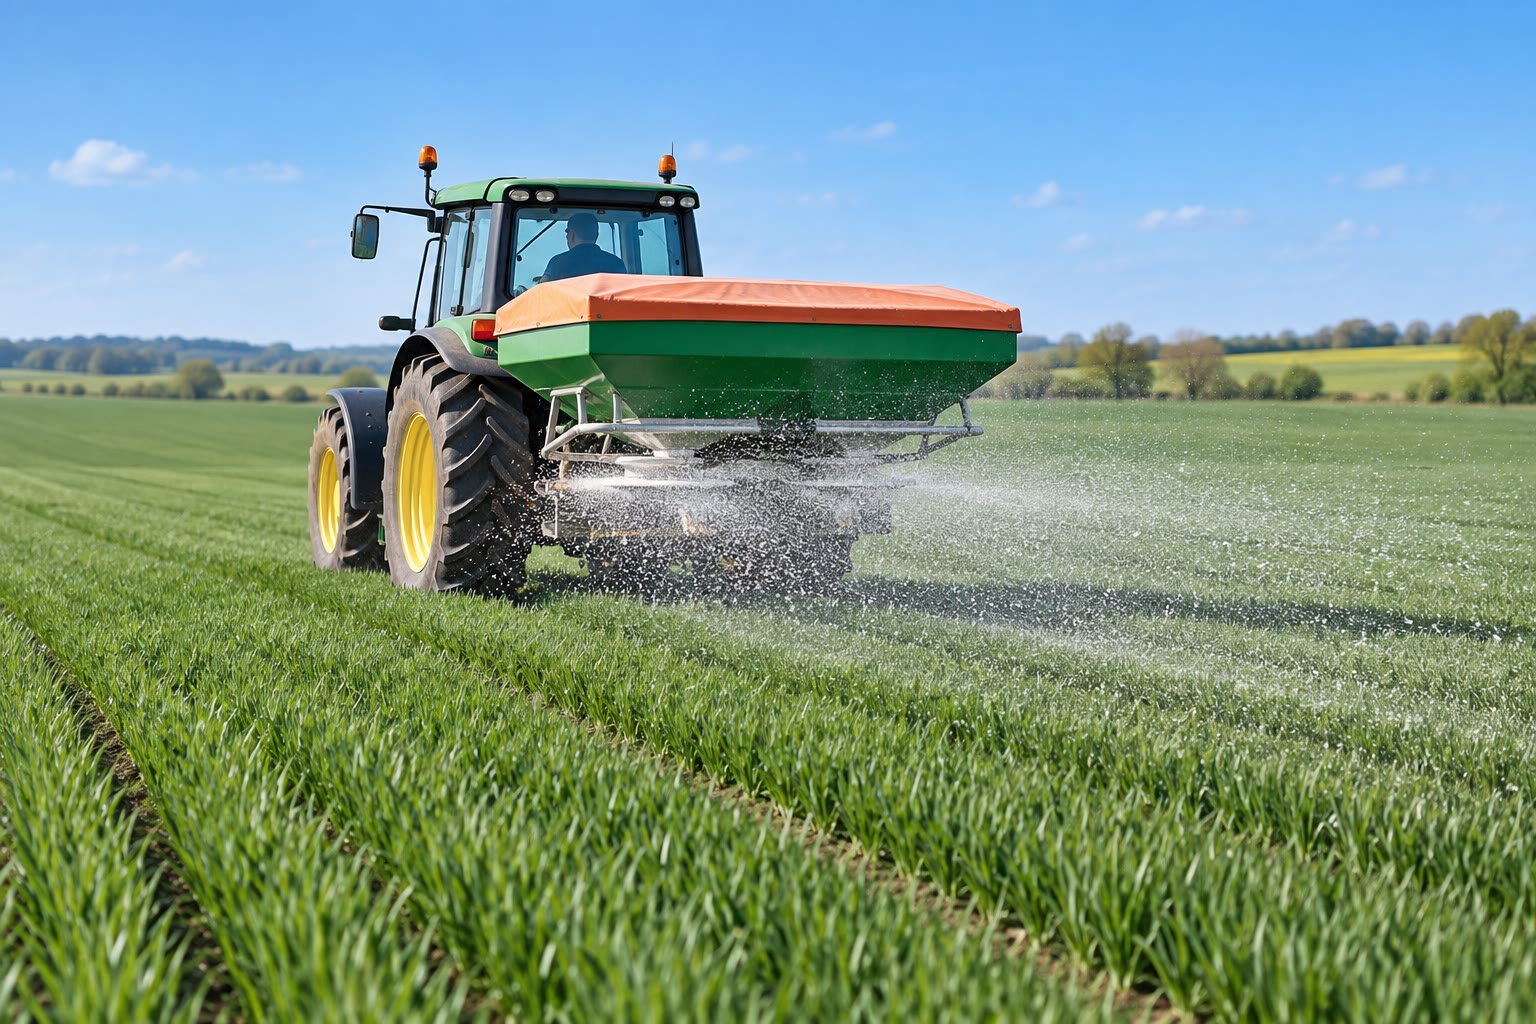
\includegraphics[width=0.55\linewidth]{images/book2/ai/b1-27-fertiliser-field.jpg}

{\small Penebaran pupuk nitrogen di ladang gandum. Sebagian besar pupuk itu
dibuat dari nitrogen udara melalui proses Haber--Bosch.}
\end{omfigure}

\section{Golongan 13: boron dan aluminium}

Boron adalah \omterm{def:b1:periodicity:metalloid}{metaloid} yang membentuk senyawa kovalen dengan oktet yang
tidak lengkap: dalam \ce{BF3} dan asam borat \ce{B(OH)3}, boron mempunyai
enam \omterm{def:b1:quantum-numbers:configuration}{elektron valensi} dan berperan sebagai \omterm{def:b1:lewis-resonance-vsepr:lewis-acid}{asam Lewis}
(\cref{ch:b1:lewis-resonance-vsepr}). Asam borat adalah \omterm{def:b1:predominant-reaction:strong-acid}{asam lemah} bukan
karena melepaskan proton, melainkan karena menerima ion hidroksida,
\ce{B(OH)3 + 2H2O <=> B(OH)4- + H3O+}. Boraks, sebuah natrium borat,
dipakai dalam kaca dan detergen.

\begin{definition}[Asam okso]\label{def:b1:p-block-13-15:oxoacid}
\emph{Asam okso}\index{asam okso} adalah asam yang atom-atom hidrogen
asamnya terikat pada atom oksigen yang terikat pada sebuah \omterm{def:b1:complexation:complex}{atom pusat}:
\ce{B(OH)3}, \ce{H2CO3}, \ce{HNO3} (\ce{HO-NO2}), \ce{H3PO4}
(\ce{(HO)3PO}), \ce{H2SO4}. Makin banyak atom oksigen tanpa hidrogen di
sekitar \omterm{def:b1:complexation:complex}{atom pusat}, makin kuat asamnya.
\end{definition}

Aluminium, di bawah boron, adalah logam, tetapi ionnya yang kecil dan
bermuatan tinggi memberinya oksida dan hidroksida yang amfoter
(\cref{sec:b1:precipitation:amphoteric}). Bijihnya adalah bauksit,
campuran aluminium hidroksida dengan oksida besi dan silika; pada tahun
2025 dunia menambang sekitar 440 juta ton bauksit dan memurnikan sekitar
150 juta ton alumina darinya.
% ledger: usgs:bauxite-world-2025, usgs:alumina-world-2025

\begin{proposition}[Proses Bayer]\label{prop:b1:p-block-13-15:bayer}
Natrium hidroksida pekat yang panas melarutkan aluminium dari bauksit
sebagai \ce{Al(OH)4-} dan meninggalkan oksida besi (lumpur merah);
pendinginan dan pembenihan larutan yang telah disaring mengendapkan
\ce{Al(OH)3} murni, yang dikalsinasi menjadi alumina,
\ce{2Al(OH)3 -> Al2O3 + 3H2O}.
\end{proposition}

\begin{proof}
\ce{Al(OH)3(s) + OH- <=> Al(OH)4-} mempunyai $K = 10^{-1.23}$ pada
\qty{25}{\celsius} (\cref{ch:b1:precipitation}): pada \ce{[OH-]} yang
tinggi, aluminium berada dalam larutan, sedangkan besi(III) hidroksida,
yang tidak amfoter, tetap padat (\cref{exo:b1:precipitation:12}).
Pengenceran dan pendinginan menurunkan \ce{[OH-]} dan menggeser kuosiennya
sehingga $Q > K$ untuk reaksi balik: hidroksidanya mengendap. Kalsinasi
mengeluarkan air.
\end{proof}

Alumina lalu direduksi menjadi aluminium melalui elektrolisis dalam
leburan kriolit, sebuah industri yang dipelajari dalam jilid Tahun~2.

\begin{omfigure}
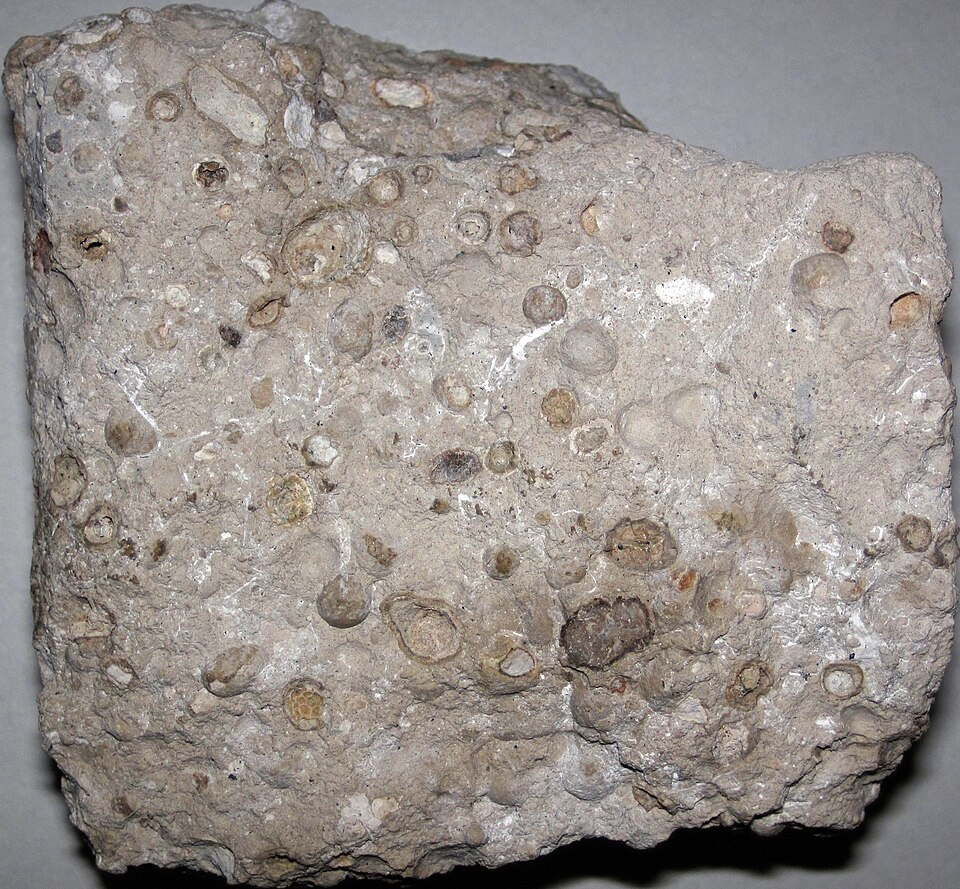
\includegraphics[height=3.6cm]{images/book2/bauxite.jpg}\hspace{0.4em}%
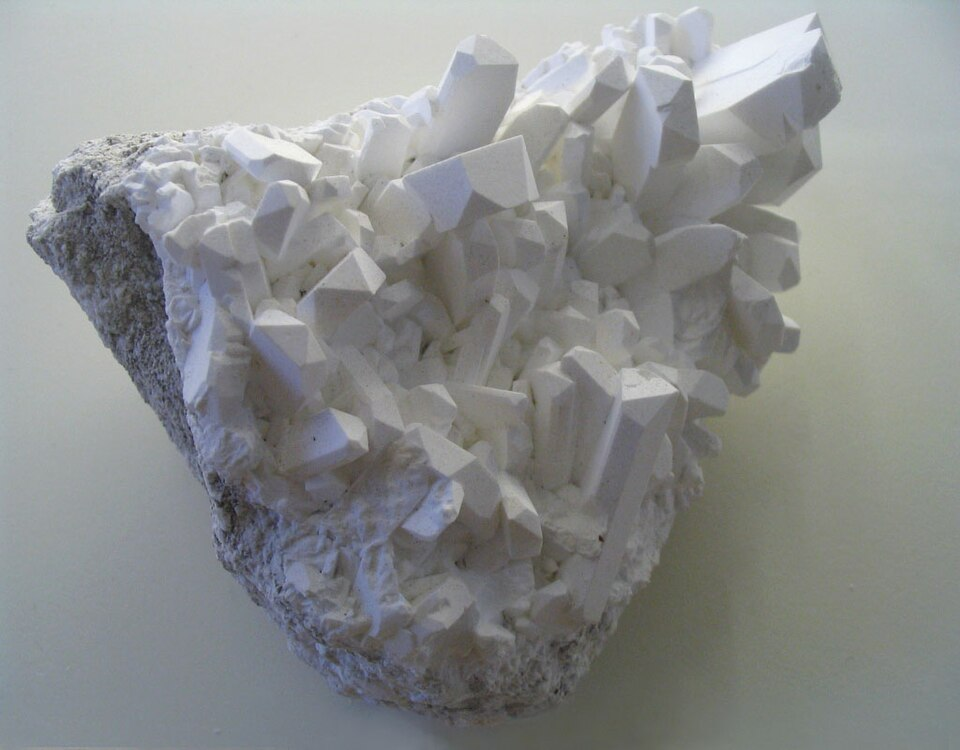
\includegraphics[height=3.6cm]{images/book2/borax.jpg}\hspace{0.4em}%
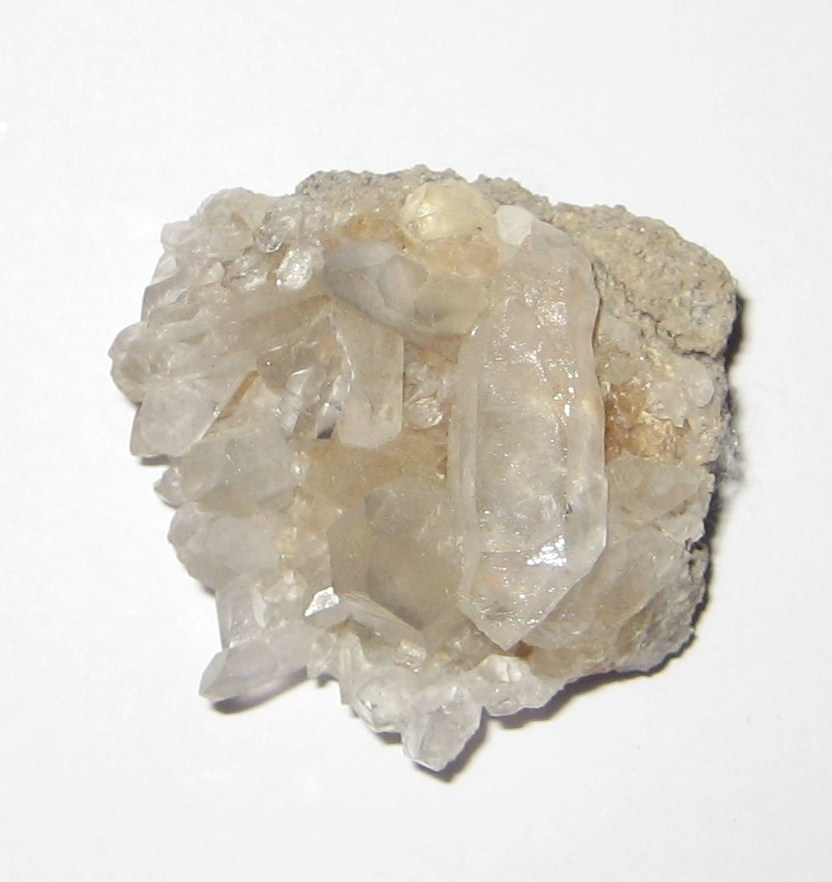
\includegraphics[height=3.6cm]{images/book2/quartz.jpg}\hspace{0.4em}%
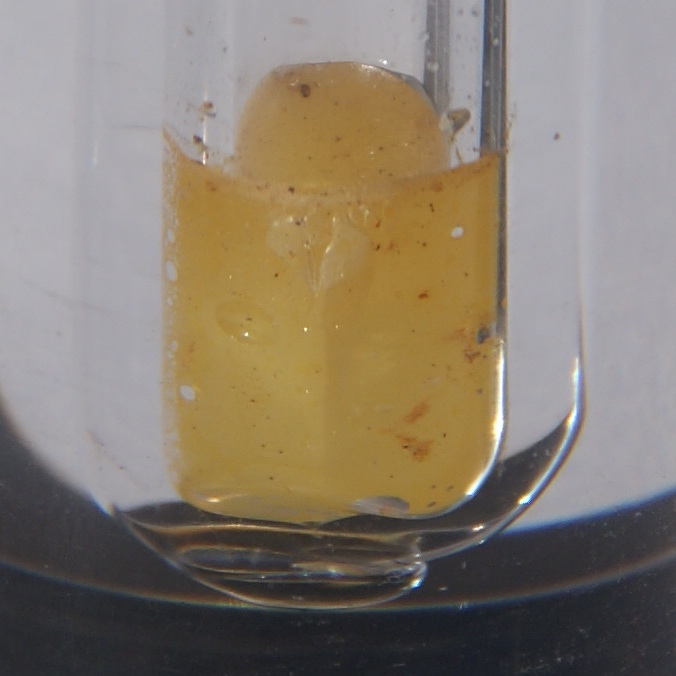
\includegraphics[height=3.6cm]{images/book2/white-phosphorus.jpg}

{\small Dari kiri ke kanan: bauksit pisolitik (James St. John, CC BY 2.0);
\omterm{def:b1:crystals-metals:crystal}{kristal} boraks (Aram Dulyan, domain publik); sekelompok \omterm{def:b1:crystals-metals:crystal}{kristal} kuarsa,
\ce{SiO2} (Stephanie Clifford, CC BY 2.0); fosfor putih, dengan sedikit
fosfor merah, disimpan di bawah air karena terbakar di udara (Hi-Res
Images of Chemical Elements, CC BY 3.0). Semuanya dari Wikimedia Commons.}
\end{omfigure}

\section{Golongan 14: karbon dan silikon}

Karbon dan silikon sama-sama membentuk empat ikatan, tetapi dengan cara
yang berbeda. Karbon membentuk ikatan rangkap dua yang kuat: \ce{CO2}
adalah molekul, \ce{O=C=O}, sebuah gas. Silikon hampir tidak melakukannya:
\ce{SiO2} adalah jaringan kovalen tetrahedron \ce{SiO4} yang berbagi semua
sudutnya, sebuah padatan keras, kuarsa (\cref{ch:b1:crystals-ionic-covalent}).
Karbon dioksida adalah \omterm{def:b1:s-block:oxide-character}{oksida asam}, yang menghasilkan asam karbonat,
hidrogenkarbonat, dan karbonat (\cref{ch:b1:predominant-reaction});
silika juga \omterm{def:b1:s-block:oxide-character}{oksida asam}, yang diserang oleh leburan alkali menghasilkan
silikat.

\begin{proposition}[Satuan silikat]\label{prop:b1:p-block-13-15:silicate-units}
Silikat tersusun atas tetrahedron \ce{SiO4}; banyaknya sudut yang dipakai
bersama dengan tetrahedron lain menentukan rumus anionnya: tidak ada,
\ce{SiO4^4-} (tetrahedron terisolasi); dua, rantai $(\ce{SiO3})_n^{2n-}$;
tiga, lembaran $(\ce{Si2O5})_n^{2n-}$; empat, kerangka netral \ce{SiO2}.
\end{proposition}

\begin{proof}
Oksigen yang dipakai bersama dimiliki setengahnya oleh setiap tetrahedron.
Tetrahedron yang berbagi
$k$ sudut memiliki $4 - k$ atom oksigen seutuhnya dan $k$ atom setengahnya: $4 -
k/2$ oksigen per silikon. Setiap oksigen yang tidak dipakai bersama
membawa muatan $-1$ (oksigen itu mempunyai satu ikatan), setiap oksigen
yang dipakai bersama tidak bermuatan: muatan per silikon adalah
$-(4 - k)$. $k = 0$: \ce{SiO4^4-}; $k = 2$: \ce{SiO3^2-} per silikon;
$k = 3$: \ce{SiO_{2.5}^-}, yaitu \ce{Si2O5^2-}; $k = 4$: \ce{SiO2}.
\end{proof}

\begin{omfigure}
\begin{tikzpicture}[font=\small, line join=round]
  % one SiO4 tetrahedron in perspective
  \begin{scope}
    \coordinate (t) at (0,1.2); \coordinate (a) at (-1.0,-0.5);
    \coordinate (b) at (1.0,-0.5); \coordinate (c) at (0.25,0.05);
    \draw[thick, omDef] (t) -- (a) -- (b) -- cycle; \draw[thick, omDef] (t) -- (b);
    \draw[dashed, omDef] (a) -- (c) -- (b) (t) -- (c);
    \foreach \p in {t,a,b,c} \shade[ball color=red!60] (\p) circle (0.16);
    \shade[ball color=gray!40] (0.06,0.18) circle (0.11);
    \node at (0,-1.2) {\ce{SiO4^4-}: satu tetrahedron};
  \end{scope}
  % a chain of tetrahedra seen from above
  \begin{scope}[xshift=3.6cm]
    \foreach \i in {0,1,2,3} {
      \draw[thick, omDef, fill=omDef!10] (\i*1.1,0) -- (\i*1.1+0.55,0.95) -- (\i*1.1+1.1,0) -- cycle;
      \shade[ball color=red!60] (\i*1.1+0.55,0.95) circle (0.12);
      \shade[ball color=red!60] (\i*1.1+0.55,0.32) circle (0.10);
    }
    \foreach \i in {0,1,2,3,4} \shade[ball color=red!60] (\i*1.1,0) circle (0.12);
    \node[align=center] at (2.2,-1.0) {rantai $(\ce{SiO3})_n^{2n-}$: setiap tetrahedron\\ berbagi dua sudut (dilihat dari atas)};
  \end{scope}
\end{tikzpicture}

{\small Satuan silikat: sebuah tetrahedron \ce{SiO4} terisolasi (silikon
abu-abu, oksigen merah), dan sebuah rantai yang setiap tetrahedronnya
berbagi dua atom oksigen dengan tetangganya. Lembaran (tiga sudut
bersama) membentuk mika dan lempung; kerangka (empat) membentuk kuarsa.}
\end{omfigure}

\begin{definition}[Efek pasangan inert]\label{def:b1:p-block-13-15:inert-pair}
\emph{Efek pasangan inert}\index{efek pasangan inert} adalah makin
stabilnya, ke bawah dalam \omterm{def:b1:periodicity:table}{golongan} 13 sampai 15, keadaan oksidasi yang
dua di bawah keadaan tertinggi \omterm{def:b1:periodicity:table}{golongannya}: talium(I) dan bukan (III),
timbal(II) dan bukan (IV), bismut(III) dan bukan (V). Pasangan
\textit{ns}$^2$ unsur-unsur berat terikat erat dan hanya sedikit ikut
serta dalam ikatan.
\end{definition}

Efek itu menjelaskan mengapa timbal(IV) oksida adalah \omterm{def:b1:nernst:couple}{oksidator} kuat
($E^\circ(\ce{PbO2}/\ce{Pb^2+}) = 1.46$~V, \cref{ch:b1:nernst}), sedangkan
karbon(IV) dan silikon(IV) adalah keadaan stabil unsur-unsurnya.

\section{Golongan 15: nitrogen}

\begin{proposition}[Tangga nitrogen]\label{prop:b1:p-block-13-15:nitrogen-ladder}
Nitrogen mengambil setiap \omterm{def:b1:nernst:oxidation-number}{bilangan oksidasi} dari $-3$ sampai $+5$: \ce{NH3} dan
\ce{NH4+} ($-$III), \ce{N2H4} ($-$II), \ce{NH2OH} ($-$I), \ce{N2} (0),
\ce{N2O} ($+$I), \ce{NO} ($+$II), \ce{HNO2} dan \ce{NO2-} ($+$III),
\ce{NO2} ($+$IV), \ce{HNO3} dan \ce{NO3-} ($+$V).
\end{proposition}

\begin{proof}
Terapkan aturan dalam \cref{prop:b1:nernst:on-rules} pada setiap rumus,
dengan H pada $+$I dan O pada $-$II: dalam \ce{N2H4}, $2x + 4 = 0$; dalam \ce{NO2-}, $x - 4 =
-1$; dan seterusnya.
\end{proof}

\begin{definition}[Fiksasi nitrogen]\label{def:b1:p-block-13-15:nitrogen-fixation}
\emph{Fiksasi nitrogen}\index{fiksasi nitrogen} adalah setiap proses yang
mengubah dinitrogen udara menjadi senyawa (amonia, nitrat) yang dapat
dipakai oleh makhluk hidup atau industri: fiksasi biologis oleh bakteri,
fiksasi oleh petir, dan sintesis amonia secara industri.
\end{definition}

Proses Haber--Bosch menggabungkan nitrogen dan hidrogen di atas \omterm{def:b1:elementary-steps:catalyst}{katalis}
besi, \ce{N2 + 3H2 <=> 2NH3}. Reaksi itu disukai pada suhu kamar
($K = 10^{5.8}$ pada \qty{25}{\celsius}, dari energi Gibbs pembentukan
amonia), tetapi terlalu lambat; \omterm{def:b1:elementary-steps:catalyst}{katalisnya} hanya bekerja dalam keadaan
panas, dan pilihan suhu dan tekanan yang mendamaikan laju dan \omterm{def:b1:extent-q-and-k:fractional-extent}{rendemen}
dibahas dalam jilid Tahun~2. Amonia lalu dioksidasi menjadi asam nitrat
melalui proses Ostwald.
% ledger: dfg:NH3_g

\begin{omfigure}
\begin{tikzpicture}[font=\small, >={Stealth}, box/.style={draw, rounded corners, fill=omDef!8, align=center, minimum height=0.9cm}]
  \node[box] (air) at (0,0) {udara\\\ce{N2}};
  \node[box] (gas) at (0,-1.6) {gas alam\\\ce{H2}};
  \node[box] (hb) at (3.4,-0.8) {Haber--Bosch\\katalis besi};
  \node[box] (ox1) at (7.3,-0.8) {kasa Pt--Rh\\\ce{NH3} $\to$ \ce{NO}};
  \node[box] (ox2) at (11.0,-0.8) {oksidasi\\absorpsi\\\ce{NO} $\to$ \ce{NO2} $\to$ \ce{HNO3}};
  \draw[->, thick] (air) -- (hb);
  \draw[->, thick] (gas) -- (hb);
  \draw[->, thick] (hb) -- node[above] {\ce{NH3}} (ox1);
  \draw[->, thick] (ox1) -- node[above] {\ce{NO}} (ox2);
  \draw[->, thick] (ox2.south) -- ++(0,-0.6) node[below] {\ce{HNO3}};
  \draw[->, thick] (hb.south) -- ++(0,-0.9) node[below] {\ce{NH3} (pupuk)};
  \draw[->, thick] (ox2.north) -- ++(0,0.5) -| node[pos=0.25, above] {\ce{NO} didaur ulang} (ox1.north);
\end{tikzpicture}

{\small Dari udara ke asam nitrat: sintesis amonia yang diikuti oleh tiga
tahap proses Ostwald.}
\end{omfigure}

\begin{method}[Menyetarakan persamaan industri yang berantai]\label{met:b1:p-block-13-15:ostwald-balance}
\begin{enumerate}
  \item Setarakan setiap tahap: (1) \ce{4NH3 + 5O2 -> 4NO + 6H2O};
        (2) \ce{2NO + O2 -> 2NO2}; (3) \ce{3NO2 + H2O -> 2HNO3 + NO}.
  \item Kalikan tahap-tahapnya sehingga setiap zat antara yang terbentuk
        juga terpakai (\ce{NO} dari tahap 3 kembali ke tahap 2).
  \item Jumlahkan: dengan daur ulang NO yang sempurna, persamaan
        keseluruhannya adalah \ce{NH3 + 2O2 -> HNO3 + H2O}, satu asam
        nitrat per amonia.
  \item Gunakan persamaan keseluruhan untuk neraca massa, dan
        tahap-tahapnya untuk rancangan setiap reaktor.
\end{enumerate}
\end{method}

\begin{history}[Fritz Haber]
\begin{minipage}[t]{0.18\linewidth}\vspace{0pt}
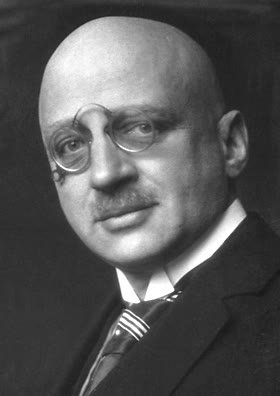
\includegraphics[width=\linewidth]{images/book2/haber.jpg}
\end{minipage}\hfill
\begin{minipage}[t]{0.78\linewidth}\vspace{0pt}
Fritz Haber menunjukkan bahwa amonia dapat dibuat dari nitrogen dan
hidrogen di bawah tekanan di atas sebuah \omterm{def:b1:elementary-steps:catalyst}{katalis}; Carl Bosch mengubah
reaksi laboratorium itu menjadi proses industri. Haber menerima Hadiah
Nobel Kimia untuk tahun 1918. Orang yang sama memimpin penggunaan klorin
pertama dalam skala besar sebagai senjata dalam Perang Dunia Pertama:
kimia yang memberi makan separuh umat manusia dan kimia yang membunuh
dipisahkan oleh pilihan para kimiawan. (Foto: Yayasan Nobel, terbit
1919, domain publik, Wikimedia Commons.)
\end{minipage}
\end{history}

\section{Fosfor dan kecenderungan ke bawah golongan}

Fosfor, di bawah nitrogen, tidak membentuk ikatan rangkap tiga \ce{P#P}:
fosfor putih tersusun atas tetrahedron \ce{P4}, yang tegang dan reaktif
(fosfor itu terbakar di udara dan disimpan di bawah air); fosfor merah
adalah polimer, yang jauh kurang reaktif. Pembakaran fosfor menghasilkan
\ce{P4O10}, oksida yang paling asam di antara oksida-oksida yang umum,
yang dengan air menghasilkan asam fosfat, $\mathrm{p}K_a$ 2.15, 7.21,
12.34 (\cref{ch:b1:predominant-reaction}). Batuan fosfat, yang ditambang
sekitar 250 juta ton pada tahun 2025, diubah oleh asam sulfat menjadi
pupuk fosfat.
% ledger: usgs:phosphate-world-2025

Ke bawah setiap \omterm{def:b1:periodicity:table}{golongan}, unsur-unsurnya makin bersifat logam (boron ke
talium, karbon ke timbal, nitrogen ke bismut), oksidanya makin basa, dan
keadaan oksidasi yang lebih rendah makin stabil: \omterm{def:b1:p-block-13-15:inert-pair}{efek pasangan inert}. Di
sepanjang \omterm{def:b1:periodicity:table}{periode}, oksida makin asam, dari \ce{Na2O} yang basa ke
oksida-oksida fosfor dan belerang yang asam.

\section{Latihan}

\begin{exercise}[$\star$]\label{exo:b1:p-block-13-15:1}
Tentukan \omterm{def:b1:nernst:oxidation-number}{bilangan oksidasi} nitrogen dalam \ce{NH4NO3} (kedua atomnya),
\ce{N2O5}, \ce{HNO2}, \ce{N2H4}, dan \ce{Mg3N2}.
\end{exercise}

\begin{exercise}[$\star$]\label{exo:b1:p-block-13-15:2}
Gambarlah \omterm{def:b1:lewis-resonance-vsepr:lewis}{struktur Lewis} \ce{BF3}, \ce{NH3}, dan senyawa adisi
\ce{F3B-NH3}; kenali \omterm{def:b1:lewis-resonance-vsepr:lewis-acid}{asam Lewis} dan \omterm{def:b1:lewis-resonance-vsepr:lewis-acid}{basa Lewisnya}.
\end{exercise}

\begin{exercise}[$\star$]\label{exo:b1:p-block-13-15:3}
Tuliskan reaksi \ce{CO2}, \ce{SiO2} (lebur), dan \ce{P4O10} dengan
natrium hidroksida, serta reaksi \ce{Al2O3} dengan asam dan dengan basa.
\end{exercise}

\begin{exercise}[$\star$]\label{exo:b1:p-block-13-15:4}
Hitunglah tetapan kesetimbangan \ce{N2 + 3H2 <=> 2NH3} pada
\qty{25}{\celsius} dari $\Delta_f G^\circ(\ce{NH3}) =
\qty{-16.45}{kJ/mol}$.
\end{exercise}

\begin{exercise}[$\star\star$]\label{exo:b1:p-block-13-15:5}
Dengan memakai cara penghitungan dalam \cref{prop:b1:p-block-13-15:silicate-units},
tentukan rumus sebuah cincin enam tetrahedron yang masing-masing berbagi
dua sudut (seperti pada beril) dan rumus sebuah rantai ganda yang
separuh tetrahedronnya berbagi dua sudut dan separuhnya lagi tiga sudut.
\end{exercise}

\begin{exercise}[$\star\star$]\label{exo:b1:p-block-13-15:6}
Hitunglah massa alumina yang diperoleh dari satu ton bauksit yang
mengandung \qty{55}{\percent} massa \ce{Al(OH)3}, dengan perolehan
\qty{92}{\percent}.
\end{exercise}

\begin{exercise}[$\star\star$]\label{exo:b1:p-block-13-15:7}
Tunjukkan bahwa asam borat adalah \omterm{def:b1:lewis-resonance-vsepr:lewis-acid}{asam Lewis} dan bukan \omterm{def:b1:predominant-reaction:bronsted}{asam Brønsted}, dan
jelaskan mengapa larutannya tetap bersifat asam.
\end{exercise}

\begin{exercise}[$\star\star$]\label{exo:b1:p-block-13-15:8}
Setarakan oksidasi amonia menjadi \ce{NO} dengan \omterm{def:b1:nernst:oxidation-number}{bilangan oksidasi} dan
tentukan banyaknya elektron yang dipertukarkan per \ce{NH3}.
\end{exercise}

\begin{exercise}[$\star\star$]\label{exo:b1:p-block-13-15:9}
Amonium nitrat dibuat dari amonia dan asam nitrat. Tuliskan reaksinya, dan
hitunglah massa amonia yang diperlukan (baik untuk asam nitratnya maupun
untuk penetralannya) per ton amonium nitrat.
\end{exercise}

\begin{exercise}[$\star\star\star$]\label{exo:b1:p-block-13-15:10}
Jelaskan mengapa nitrogen adalah gas diatomik dan fosfor adalah padatan
yang tersusun atas molekul \ce{P4}, dan mengapa karbon dioksida adalah
gas dan silika padatan, dengan memakai kekuatan ikatan $\pi$ antara
atom-atom \omterm{def:b1:periodicity:table}{periode} kedua dan \omterm{def:b1:periodicity:table}{periode} ketiga.
\end{exercise}

\begin{exercise}[$\star\star\star$]\label{exo:b1:p-block-13-15:11}
Tunjukkan dengan \omterm{def:b1:nernst:electrode-potential}{potensial standar} bahwa timbal(IV) oksida mengoksidasi
ion klorida menjadi klorin dalam asam, sedangkan silikon(IV) oksida tidak
melakukan hal semacam itu. Hubungkan hal ini dengan \omterm{def:b1:p-block-13-15:inert-pair}{efek pasangan inert}.
\end{exercise}

\begin{exercise}[$\star\star\star$]\label{exo:b1:p-block-13-15:12}
Dunia memproduksi sekitar 160 juta ton nitrogen dalam bentuk amonia pada
tahun 2025. Berapa massa amonia itu, dan berapa massa hidrogen yang
dikandungnya? Dari mana sebagian besar hidrogen itu berasal?
\end{exercise}

\section{Soal: Dari Udara ke Pupuk}

\begin{problem}[{Soal akhir pekan --- ikatan rangkap tiga nitrogen,
sintesis amonia, tiga tahap pembuatan asam nitrat, amonium nitrat, dan
massa asam nitrat yang dapat diperoleh dari satu ton amonia}]
\label{pb:b1:p-block-13-15:1}
Sebuah pabrik pupuk mengubah amonia menjadi asam nitrat dan amonium
nitrat. Massa molar (\unit{g/mol}): \ce{N2} 28.0, \ce{H2} 2.0, \ce{NH3}
17.0, \ce{HNO3} 63.0, \ce{NH4NO3} 80.0, \ce{O2} 32.0;
$\Delta_f G^\circ(\ce{NH3(g)}) = \qty{-16.45}{kJ/mol}$ pada
\qty{25}{\celsius}.

\medskip
\noindent\textbf{Bagian I --- Nitrogen.}
\begin{enumerate}
  \item Gambarlah \omterm{def:b1:lewis-resonance-vsepr:lewis}{struktur Lewis} \ce{N2} dan jelaskan mengapa zat itu
        tidak reaktif.
  \item Tentukan \omterm{def:b1:nernst:oxidation-number}{bilangan oksidasi} N dalam \ce{N2}, \ce{NH3}, \ce{NO},
        \ce{NO2}, \ce{HNO3}, dan \ce{NH4NO3}.
  \item Sebutkan tiga cara alami atau industri untuk memfiksasi nitrogen.
  \item Mengapa tumbuhan tidak dapat memakai \ce{N2} secara langsung?
  \item Unsur manakah yang dioksidasi dan manakah yang direduksi dalam
        sintesis amonia?
  \item Tuliskan sintesis amonia.
\end{enumerate}

\medskip
\noindent\textbf{Bagian II --- Amonia.}
\begin{enumerate}[resume]
  \item Hitunglah tetapan kesetimbangan sintesis itu pada
        \qty{25}{\celsius}.
  \item Mengapa sintesis itu tetap dijalankan dalam keadaan panas, di atas
        sebuah \omterm{def:b1:elementary-steps:catalyst}{katalis}?
  \item Hitunglah massa \ce{N2} dan \ce{H2} untuk satu ton amonia.
  \item Berapa volume udara (\qty{78}{\percent} volume \ce{N2}, gas ideal,
        \qty{25}{\celsius}, \qty{1}{bar}) yang mengandung nitrogen itu?
  \item Dari mana hidrogennya berasal?
  \item Mengapa amonia sendiri dipakai sebagai pupuk di beberapa negara,
        dan mengapa amonia sering diubah lebih dahulu?
\end{enumerate}

\medskip
\noindent\textbf{Bagian III --- Asam nitrat.}
\begin{enumerate}[resume]
  \item Setarakan tahap 1, \ce{NH3 + O2 -> NO + H2O}, dengan \omterm{def:b1:nernst:oxidation-number}{bilangan oksidasi}. % ce-unbalanced-ok
  \item Setarakan tahap 2, \ce{NO + O2 -> NO2}. % ce-unbalanced-ok
  \item Setarakan tahap 3, \ce{NO2 + H2O -> HNO3 + NO}. Reaksi redoks % ce-unbalanced-ok
        jenis apakah itu?
  \item Gabungkan tahap-tahapnya dengan daur ulang NO yang sempurna
        menjadi persamaan keseluruhan.
  \item Hitunglah massa oksigen yang terpakai per ton amonia.
  \item Mengapa dipakai kasa platina--rodium pada tahap 1?
\end{enumerate}

\medskip
\noindent\textbf{Bagian IV --- Amonium nitrat dan neraca massa.}
\begin{enumerate}[resume]
  \item Tuliskan pembentukan amonium nitrat.
  \item Berapa bagian amonia yang harus diubah menjadi asam nitrat agar
        hanya dihasilkan amonium nitrat?
  \item Hitunglah massa amonium nitrat dari satu ton amonia yang dibagi
        dengan cara itu.
  \item Berapa persen nitrogen yang dikandung amonium nitrat?
  \item Mengapa amonium nitrat harus disimpan jauh dari bahan bakar dan
        kalor?
  \item Hitunglah massa asam nitrat yang dapat diperoleh dari satu ton
        amonia (konversi sempurna).
\end{enumerate}
\end{problem}
